\documentclass[aspectratio=169,10pt]{beamer}
%\usepackage{zxjatype}
%\usepackage[ipaex]{zxjafont}

\usepackage{fontspec}
\usepackage{polyglossia}
\usepackage{anyfontsize}
\usepackage{fancyvrb}
\usepackage{multirow}
\usepackage{arydshln}

\usepackage{makeidx}
\makeindex

\setdefaultlanguage{japanese}
%\setromanfont{Noto Serif}
%\setmainfont{Noto Serif}
%\setsansfont{Noto Serif}
\setmainfont{Noto Serif CJK JP}[Language=Japanese,Script=CJK]
\setsansfont{Noto Sans CJK JP}[Language=Japanese,Script=CJK]
\setmonofont{Noto Sans Mono CJK JP}
%\setmainfont{DejaVu Sans}
%\setsansfont{DejaVu Sans}

%\newfontfamily\englishfont{Noto Serif}
\newfontfamily\englishfont{DejaVu Sans}
\setotherlanguage{english}
\newfontfamily\japanesefont{Noto Serif CJK JP}[Language=Japanese,Script=CJK]
\newfontfamily\koreanfont{Noto Serif CJK KR}[Language=Korean,Script=Hangul]
\setotherlanguage{korean}
\newfontfamily\thaifont{Noto Serif Thai}[Language=Thai,Script=Thai]
%\newfontfamily\thaifont{DejaVu Sans}[Script=Thai]
\setotherlanguage{thai}
\newfontfamily\hebrewfont{Noto Serif Hebrew}[Script=Hebrew]
%\newfontfamily\hebrewfont{DejaVu Sans}[Script=Hebrew]
%\newfontfamily\hebrewfont{DejaVu Sans}
%\newfontfamily\hebrewfont{SILEOT.ttf}[Script=Hebrew]
\setotherlanguage{hebrew}
%\newfontfamily\arabicfont{Noto Naskh Arabic}[Script=Arabic]
\newfontfamily\arabicfont{DejaVu Sans}[Script=Arabic]
\setotherlanguage{arabic}

\usetheme{Copenhagen}
%\usetheme{CambridgeUS}
%\usetheme{Berlin}
%\usetheme{Boadilla}
%\usetheme{Madrid}
%\usetheme{Antibes}
%\usetheme{Montpellier}
%\usetheme{Berkeley}
%\usetheme{Goettingen}
\usetheme{Singapore}%% 候補
%\usetheme{Szeged}
\usecolortheme{seahorse}%% 候補

\newcommand{\colRd}{\color{purple}}
\newcommand{\colBk}{\color{black}}
\newcommand{\colGy}{\color{darkgray}}
\newcommand{\colGn}{\color{teal}}
\newcommand{\colBl}{\color{blue}}
%\newcommand{\verbVS}{\vspace*{-2.5ex}}
\newcommand{\exclamation}{!}


\title{\textjapanese{upmendexで作る多言語索引}\\
~Multilingual index processing by upmendex}

\author{田中 琢爾\\~TANAKA Takuji}

\begin{document}
\year=2022\month=11\day=19

\begin{japanese}
\frame{\titlepage}
\end{japanese}

\section{Overview}
\begin{frame}{Overview}

\begin{columns}
\begin{column}{70mm}

  \begin{itemize}
  \item Feature of \textbf{upmendex}\\
     --- Multilingual index processor
  \item Treatment for Scripts
     \begin{itemize}
      \item Latin, Cyrillic, Greek
      \item CJK (Chinese, Japanese, Korean)
      \item Devanagari, Thai, Arabic, Hebrew
      \item Symbol, Number
     \end{itemize}
  \item Multilingual environment
  \item Benchmark
  \end{itemize}
\end{column}

\begin{column}{65mm}

\begin{center}
\fbox{%
  \includegraphics[scale=0.47]{city_texconf-03-cropa.pdf}%
}
\end{center}
\end{column}
\end{columns}

\end{frame}
\subsection{Feature of upmendex}
\begin{frame}{Feature of upmendex~~{\scriptsize (Ver. 1.05)}}
\renewcommand{\thefootnote}{$\dagger$}
  \begin{itemize}
  \item Index processor
    \begin{itemize}
    \item Upper compatible with \textbf{MakeIndex}/\textbf{Mendex}
    \item Work with upLaTeX/LuaLaTeX/XeLaTeX\\
          \hspace{15mm}\& babel/polyglossia
    \end{itemize}
  \item Localization
    \begin{itemize}
    \item Support Languages / Scripts
      \begin{itemize}
      \item Latin (incl. non-English), Cyrillic, Greek
      \item CJK (Chinese, Japanese, Korean)
      \item Devanagari, Thai
      \item Arabic, Hebrew
      \item Symbol, Number
      \end{itemize}
    \end{itemize}
  \item Multilingualization
    \begin{itemize}
    \item Unicode, UTF-8
    \item ICU\footnotemark{} (Collation / Upper/Lowercase)
    \item Flexible customization
    \end{itemize}
  \end{itemize}
\vspace{3mm}
{\footnotesize $\dagger$ ICU: International Components for Unicode}
%\footnotetext[1]{International Components for Unicode}
\end{frame}

% - - % - - % - - % - - % - - % - - % - - % - - % - - %

\subsection{Script, Language, Locale}

%\setmonofont{Noto Sans Mono CJK TC}
\begin{frame}[fragile]{Language, Script, Locale}

\setlength\dashlinedash{0.5pt}
\setlength\dashlinegap{1.0pt}

\begin{columns}
\begin{column}{70mm}
\footnotesize
\begin{center}
\begin{tabular}{ccc}
  Language  & Script / Index             & ICU locale \\\hline\hline
  English   & Latin                      & root           \\
  Spanish   & Latin                      & es             \\
  German    & Latin                      & de             \\
  Turkish   & Latin                      & tr             \\
  \ldots    &                            &                \\\hdashline
  Russian   & Cyrillic                   & ru             \\
  Ukrainian & Cyrillic                   & uk             \\
  \ldots    &                            &                \\\hdashline
  Greek     & Greek                      & el             \\\hline
  \multirow{4}{*}{Chinese}   & Hanzi / Pinyin         & zh             \\
            & Hanzi       / Stroke         & zh-u-co-stroke \\
            & Hanzi       / Radical-Stroke & zh-u-co-unihan \\
            & Hanzi       / Zhuyin         & zh-u-co-zhuyin \\\hdashline
  Japanese  & Kana \& Hanzi / Kana       & ja             \\\hdashline
  Korean    & Hangul                     & ko             \\\hline
\end{tabular}
\end{center}
\end{column}
\begin{column}{58mm}
\footnotesize
\begin{center}
\begin{tabular}{ccc}
  Language  & Script / Index & ICU locale \\\hline\hline
  Hindi     & Devanagari     & hi             \\
  Marathi   & Devanagari     & mr             \\
  \ldots    &                &                \\\hdashline
  Thai      & Thai           & th             \\\hline
  Persian   & Arabic         & fa             \\
  Arabic    & Arabic         & ar             \\
  \ldots    &                &                \\\hdashline
  Hebrew    & Hebrew         & he             \\
  Yiddish   & Hebrew         & yi             \\\hline
  \multirow{2}{*}{Common}  & Symbol   &       \\
            & Number         &                \\\hline
\end{tabular}
\end{center}
\textbf{upmendex} supports 60 languages,\\12 scripts \& 95 locales.
\end{column}
\end{columns}
%\vskip2ex
\end{frame}

% - - % - - % - - % - - % - - % - - % - - % - - % - - %

\section{Scripts}
\subsection{Latin, Cyrillic, Greek}
\begin{frame}{Latin, Cyrillic, Greek}
  \begin{itemize}
    \item Sorting (Collation) | ソート順
    \item Diacritical mark | ダイアクリティカルマーク
    \item Digraph/Trigraph | ダイグラフ/トライグラフ
  \end{itemize}
\end{frame}

% - - % - - % - - % - - % - - % - - % - - % - - % - - %

\setmonofont{Noto Sans Mono}
\begin{frame}[fragile]{German, Phonebook Sort Order}

\begin{columns}
\begin{column}{55mm}

\setmonofont{Noto Sans Mono}
\begin{block}{Collation Rule~~\scriptsize locale: de-u-co-phonebk}
\begin{Verbatim}[%
  fontfamily=tt,
  fontsize=\fontsize{8.0}{8.0},
  commandchars=!<>]
&!colRd!-AE<<ä<<<Ä
&OE<<ö<<<Ö
&UE<<ü<<<Ü
!colGy!-...
\end{Verbatim}
\end{block}
\begin{exampleblock}{German Inputs in *.tex}
\begin{Verbatim}[%
  fontfamily=tt,
  fontsize=\fontsize{8.0}{8.0},
  commandchars=!<>]
ad\index{ad}.
AD\index{AD}.
ae\index{!colRd!-ae!colBk!-}.
AE\index{!colRd!-AE!colBk!-}.
ä\index{!colRd!-ä!colBk!-}.
Ä\index{!colRd!-Ä!colBk!-}.
af\index{af}.
AF\index{AF}.
!colGy!-...
\end{Verbatim}
\end{exampleblock}
\end{column}

\begin{column}{38mm}
\begin{center}
\fbox{%
  \includegraphics[scale=0.48]{de00a-02-crop.pdf}%
}\\[2mm]%
default
\end{center}
\end{column}

\begin{column}{38mm}
\begin{center}
\fbox{%
  \includegraphics[scale=0.48]{de00b-02-crop.pdf}%
}\\[2mm]%
phonebook sort order
\end{center}
\end{column}
\end{columns}

\end{frame}

% - - % - - % - - % - - % - - % - - % - - % - - % - - %

\begin{frame}[fragile]{Lithuanian, Sort Order of Y}

\begin{columns}
\begin{column}{60mm}

\setmonofont{Noto Sans Mono}
\begin{block}{Collation Rule~~\scriptsize locale: lt}
\begin{Verbatim}[%
  fontfamily=tt,
  fontsize=\fontsize{8.0}{8.0},
  commandchars=!<>]
&!colRd!-I<<į<<<Į<<y<<<Y
!colGy!-...
\end{Verbatim}
\end{block}
\begin{exampleblock}{Lithuanian Inputs in *.tex}
\begin{Verbatim}[%
  fontfamily=tt,
  fontsize=\fontsize{8.0}{8.0},
  commandchars=!<>]
i\index{i}.
I\index{I}.
į\index{į}.
Į\index{Į}.
y\index{y}.
Y\index{Y}.
!colGy!-...
\end{Verbatim}
\end{exampleblock}
\end{column}

\begin{column}{60mm}
\begin{center}
\fbox{%
  \includegraphics[scale=0.48]{lt00-02-crop.pdf}%
}%
\end{center}
\end{column}
\end{columns}

\end{frame}

% - - % - - % - - % - - % - - % - - % - - % - - % - - %

\begin{frame}[fragile]{Slovak, Diacritical Mark}

\begin{columns}
\begin{column}{55mm}

\setmonofont{Noto Sans Mono}
\begin{block}{Collation Rule~~\scriptsize locale: sk}
\begin{Verbatim}[%
  fontfamily=tt,
  fontsize=\fontsize{8.0}{8.0},
  commandchars=!<>]
&!colRd!-O<ô<<<Ô
!colGy!-...
\end{Verbatim}
\end{block}
\begin{block}{Collation Rule~~\scriptsize locale: sk-u-co-search}
\begin{Verbatim}[%
  fontfamily=tt,
  fontsize=\fontsize{8.0}{8.0},
  commandchars=!<>]
&!colRd!-L<ĺ<<<Ĺ<ľ<<<Ľ
&!colRd!-O<ó<<<Ó<ô<<<Ô
!colGy!-...
\end{Verbatim}
\end{block}
\begin{exampleblock}{Slovak Inputs in *.tex}
\begin{Verbatim}[%
  fontfamily=tt,
  fontsize=\fontsize{8.0}{8.0},
  commandchars=!<>]
l\index{l}.
ĺ\index{ĺ}.
ľ\index{ľ}.
o\index{o}.
ó\index{ó}.
ô\index{ô}.
\end{Verbatim}
\end{exampleblock}
\end{column}

\begin{column}{38mm}
\begin{center}
\fbox{%
  \includegraphics[scale=0.48]{sk00a-02-crop.pdf}%
}\\[2mm]%
default
\end{center}
\end{column}

\begin{column}{38mm}
\begin{center}
\fbox{%
  \includegraphics[scale=0.48]{sk00b-02-crop.pdf}%
}\\[2mm]%
General-Purpose Search
\end{center}
\end{column}
\end{columns}

\end{frame}

% - - % - - % - - % - - % - - % - - % - - % - - % - - %

\begin{frame}[fragile]{Turkish, Dotless / Dotted I}

\begin{columns}
\begin{column}{47mm}
\setmainfont{Noto Serif}
\setsansfont{Noto Sans}
%\begin{center}
\normalsize
\begin{tabular}{c|cc}
language & upper & lower \\\hline\hline
\multirow{2}{*}{Turkish}
        & İ & i \\
        & I & ı \\\hline
English & I & i \\
\end{tabular}
%\end{center}
\end{column}

\begin{column}{43mm}
\setmonofont{Noto Sans}
\begin{block}{Collation Rule~~\scriptsize locale: tr}
\begin{Verbatim}[%
  fontfamily=tt,
  fontsize=\fontsize{8.0}{8.0},
  commandchars=!<>]
&[before 1]!colRd!-i<ı<<<I
&!colRd!-i<<<İ
!colGy!-...
\end{Verbatim}
\end{block}
\begin{exampleblock}{Turkish Inputs in *.tex}
\begin{Verbatim}[%
  fontfamily=tt,
  fontsize=\fontsize{8.0}{8.0},
  commandchars=!<>]
h\index{h}.
H\index{H}.
i\index{i}.
ı\index{!colRd!-ı!colBk!-}.
I\index{I}.
İ\index{!colRd!-İ!colBk!-}.
j\index{j}.
J\index{J}.
!colGy!-...
\end{Verbatim}
\end{exampleblock}
\end{column}

\begin{column}{43mm}
\begin{center}
\fbox{%
  \includegraphics[scale=0.48]{tr00-02-crop.pdf}%
}\\[2mm]%
Turkish
\end{center}
\end{column}
\end{columns}

\end{frame}

% - - % - - % - - % - - % - - % - - % - - % - - % - - %

\begin{frame}[fragile]{Hungarian, Digraphs and Trigraph}

\begin{columns}
\begin{column}{60mm}

\setmonofont{Noto Sans Mono}
\begin{block}{Collation Rule~~\scriptsize locale: hu}
\begin{Verbatim}[%
  fontfamily=tt,
  fontsize=\fontsize{8.0}{8.0},
  commandchars=!<>]
&!colRd!-C<cs!colBk!-<<<Cs<<<CS
&!colRd!-D<dz!colBk!-<<<Dz<<<DZ
&!colRd!-DZ<dzs!colBk!-<<<Dzs<<<DZS
!colGy!-...
\end{Verbatim}
\end{block}
\begin{exampleblock}{Hungarian Inputs in *.tex}
\begin{Verbatim}[%
  fontfamily=tt,
  fontsize=\fontsize{8.0}{8.0},
  commandchars=!<>]
cr\index{cr}.
cs\index{!colRd!-cs!colBk!-}.
ct\index{ct}.
dy\index{dy}.
dz\index{!colRd!-dz!colBk!-}.
dzr\index{dzr}.
dzs\index{!colRd!-dzs!colBk!-}.
dzt\index{dzt}.
e\index{e}.
!colGy!-...
\end{Verbatim}
\end{exampleblock}
\end{column}

\begin{column}{60mm}
\begin{center}
\fbox{%
  \includegraphics[scale=0.48]{hu00-02-crop.pdf}%
}%
\end{center}
\end{column}
\end{columns}

\end{frame}

% - - % - - % - - % - - % - - % - - % - - % - - % - - %

\begin{frame}[fragile]{Cyrillic \& Greek}

\begin{columns}
\begin{column}{50mm}

\setmonofont{Noto Sans Mono}
\begin{exampleblock}{Russian Inputs in *.tex}
\begin{Verbatim}[%
  fontfamily=tt,
  fontsize=\fontsize{8.0}{8.0},
  commandchars=!<>]
цветок\index{цветок}.
птица\index{птица}.
ветер\index{ветер}.
луна\index{луна}.
\end{Verbatim}
\end{exampleblock}

\begin{exampleblock}{Greek Inputs in *.tex}
\begin{Verbatim}[%
  fontfamily=tt,
  fontsize=\fontsize{8.0}{8.0},
  commandchars=!<>]
λουλούδι\index{λουλούδι}.
πουλί\index{πουλί}.
άνεμος\index{άνεμος}.
φεγγάρι\index{φεγγάρι}.
\end{Verbatim}
\end{exampleblock}
\end{column}

\begin{column}{42mm}
\begin{center}
\fbox{%
  \includegraphics[scale=0.48]{ru00-02-crop.pdf}%
}\\[2mm]%
Russian
\end{center}
\end{column}

\begin{column}{42mm}
\begin{center}
\fbox{%
  \includegraphics[scale=0.48]{el00-02-crop.pdf}%
}\\[2mm]%
Greek
\end{center}
\end{column}
\end{columns}

\end{frame}

% - - % - - % - - % - - % - - % - - % - - % - - % - - %

\subsection{CJK (Chinese, Japanese, Korean)}

\setmonofont{Noto Sans Mono CJK TC}
\begin{frame}[fragile]{Chinese, Han Ideograph Sort Order}

\begin{center}

\begin{columns}

\begin{column}{77mm}
\begin{exampleblock}{Style File *.ist~~\scriptsize locale: zh-u-co-unihan}
\begin{Verbatim}[%
  fontfamily=tt,
  fontsize=\fontsize{8.0}{8.0},
  commandchars=!<>]
!colGy!-%icu_locale "zh"
!colGy!-%icu_locale "zh-u-co-stroke"
!colRd!-icu_locale "zh-u-co-unihan"
!colGy!-%icu_locale "zh-u-co-zhuyin"
hanzi_head  "一部;丨部;丶部;丿部;乙部;亅部;二部;亠部;
!colGy!-...
\end{Verbatim}
\end{exampleblock}
\end{column}

\begin{column}{60mm}
\begin{exampleblock}{Chinese Inputs in *.tex}
\begin{Verbatim}[%
  fontfamily=tt,
  fontsize=\fontsize{8.0}{8.0},
  commandchars=!<>]
花\index{花 (8, 艸, huā, ㄏㄨㄚ)}
鳥\index{鳥 (11, 鳥, niǎo, ㄋㄧㄠˇ)}
風\index{風 (9, 風, fēng, ㄈㄥ)}
月\index{月 (4, 月, yuè, ㄩㄝˋ)}
\end{Verbatim}
\end{exampleblock}
\end{column}
\end{columns}
\vskip2ex
\begin{tabular}{cc|c}
\multicolumn{2}{c|}{sort order} & locale \\\hline
Pinyin         & 拼音 & zh \\
Stroke         & 筆畫數 & zh-u-co-stroke\\
Radical-Stroke & 部首筆畫數 & zh-u-co-unihan \\
Zhuyin (Bopomofo) & 注音符號 & zh-u-co-zhuyin
\end{tabular}
\end{center}

\end{frame}

% - - % - - % - - % - - % - - % - - % - - % - - % - - %

\begin{frame}[fragile]{Chinese, Han Ideograph Sort Order}
\begin{columns}
\begin{column}{73mm}
\begin{exampleblock}{Pinyin {\footnotesize Sort Order~~拼音~~\scriptsize locale: zh}}
\makeatletter
%\def\verbatim@font{\footnotesize\textjapanese}
\def\verbatim@font{\fontsize{7.5}{7.5}\selectfont\textjapanese}
\makeatother
\begin{Verbatim}[%
  fontfamily=tt,
  fontsize=\fontsize{7.5}{7.5},
  commandchars=!<>]
\centerline{\bfseries --- !colRd!-F!colBk!- ---}\par\nobreak
  \item 風 (9, 風, !colRd!-fēng!colBk!-, ㄈㄥ)\leaders\hbox{ }\hfill 1

  \indexspace

\centerline{\bfseries --- !colRd!-H!colBk!- ---}\par\nobreak
  \item 花 (8, 艸, !colRd!-huā!colBk!-, ㄏㄨㄚ)\leaders\hbox{ }\hfill 1
\end{Verbatim}
\end{exampleblock}
\begin{exampleblock}{Stroke {\footnotesize Sort Order~~筆畫數~~\scriptsize zh-u-co-stroke}}
\makeatletter
%\def\verbatim@font{\footnotesize\textjapanese}
\def\verbatim@font{\fontsize{7.5}{7.5}\selectfont\textjapanese}
\makeatother
\begin{Verbatim}[%
  fontfamily=tt,
  fontsize=\fontsize{7.5}{7.5},
  commandchars=!<>]
\centerline{\bfseries --- !colRd!-四畫!colBk!- ---}\par\nobreak
  \item 月 (!colRd!-4!colBk!-, 月, yuè, ㄩㄝˋ)\leaders\hbox{ }\hfill 1

  \indexspace

\centerline{\bfseries --- !colRd!-八畫!colBk!- ---}\par\nobreak
  \item 花 (!colRd!-8!colBk!-, 艸, huā, ㄏㄨㄚ)\leaders\hbox{ }\hfill 1
\end{Verbatim}
\end{exampleblock}
\end{column}
\begin{column}{73mm}
\begin{exampleblock}{Radical-Stroke {\footnotesize Sort Order~~部首筆畫數~~\scriptsize zh-u-co-unihan}}
\begin{Verbatim}[%
  fontfamily=tt,
  fontsize=\fontsize{7.5}{7.5},
  commandchars=!<>]
\centerline{\bfseries --- !colRd!-月部!colBk!- ---}\par\nobreak
  \item 月 (4, !colRd!-月!colBk!-, yuè, ㄩㄝˋ)\leaders\hbox{ }\hfill 1

  \indexspace

\centerline{\bfseries --- !colRd!-艸部!colBk!- ---}\par\nobreak
  \item 花 (8, !colRd!-艸!colBk!-, huā, ㄏㄨㄚ)\leaders\hbox{ }\hfill 1
\end{Verbatim}
\end{exampleblock}
\begin{exampleblock}{Zhuyin {\footnotesize (Bopomofo) Sort Order~~注音符號~~\scriptsize zh-u-co-zhuyin}}
\makeatletter
%\def\verbatim@font{\footnotesize\textjapanese}
\def\verbatim@font{\fontsize{7.5}{7.5}\selectfont\textjapanese}
\makeatother
\begin{Verbatim}[%
  fontfamily=tt,
  fontsize=\fontsize{7.5}{7.5},
  commandchars=!<>]
\centerline{\bfseries --- !colRd!-ㄈ!colBk!- ---}\par\nobreak
  \item 風 (9, 風, fēng, !colRd!-ㄈㄥ!colBk!-)\leaders\hbox{ }\hfill 1

  \indexspace

\centerline{\bfseries --- !colRd!-ㄋ!colBk!- ---}\par\nobreak
  \item 鳥 (11, 鳥, niǎo, !colRd!-ㄋㄧㄠˇ!colBk!-)\leaders\hbox{ }\hfill
\end{Verbatim}
\end{exampleblock}
\end{column}
\end{columns}
\end{frame}

% - - % - - % - - % - - % - - % - - % - - % - - % - - %

\begin{frame}[fragile]{Chinese, Han Ideograph Sort Order}

\begin{columns}

\begin{column}{38mm}
\begin{center}
\fbox{%
  \includegraphics[scale=0.48]{zh00a-02-crop.pdf}%
}\\[2mm]%
拼音\\
pinyin
\end{center}
\end{column}

\begin{column}{38mm}
\begin{center}
\fbox{%
  \includegraphics[scale=0.48]{zh00b-02-crop.pdf}%
}\\[2mm]%
筆畫數\\
stroke
\end{center}
\end{column}

\begin{column}{38mm}
\begin{center}
\fbox{%
  \includegraphics[scale=0.48]{zh00c-02-crop.pdf}%
}\\[2mm]%
部首筆畫數\\
radical-stroke
\end{center}
\end{column}

\begin{column}{38mm}
\begin{center}
\fbox{%
  \includegraphics[scale=0.48]{zh00d-02-crop.pdf}%
}\\[2mm]%
注音符號\\
zhuyin (bopomofo)
\end{center}
\end{column}
\end{columns}

\end{frame}

% - - % - - % - - % - - % - - % - - % - - % - - % - - %

\setmonofont{Noto Sans Mono CJK JP}[Language=Japanese,Script=CJK]
\begin{frame}[fragile]{Japanese, Sort by Reading (yomi)}

\begin{columns}
\begin{column}{85mm}
\begin{exampleblock}{Japanese Inputs with Reading {\footnotesize(Yomi)} in *.tex}
\begin{Verbatim}[%
  fontfamily=tt,
  fontsize=\fontsize{8.0}{8.0},
  commandchars=!<>]
\newcommand{\YomiTag}[1]{\relax}

%%  \index{!colRd!-reading!colBk!-@!colRd!-index_word!colBk!-}
生酒\index{なまざけ@生酒}。
生一本\index{きいっぽん@生一本}。
生け簀\index{いけす@生け簀}。
生絹\index{きぎぬ@生絹\YomiTag{きぎぬ}}%
    \index{すずし@生絹\YomiTag{すずし}}。
生飯\index{さば@生飯}。
生姜\index{しょうが@生姜}。
生活\index{せいかつ@生活\YomiTag{せいかつ}}
    \index{たつき@生活\YomiTag{たつき}}。
!colGy!-...
\end{Verbatim}
\end{exampleblock}
%\vspace{2mm}
{\footnotesize Hanzi/Kana words are sorted by reading (yomi), indexed by Kana.}\\
{\footnotesize This feature is implemented by \textbf{ASCII mendex}.}
\end{column}

\begin{column}{50mm}
\begin{center}
\fbox{%
  \includegraphics[scale=0.48]{yomi01-02-crop.pdf}%
}%
\end{center}
\end{column}
\end{columns}

\end{frame}

% - - % - - % - - % - - % - - % - - % - - % - - % - - %

\begin{frame}[fragile]{Japanese, Reading (yomi) \& Dictionary}

\begin{columns}
\begin{column}{70mm}
\begin{exampleblock}{Japanese Inputs in *.tex}
\begin{Verbatim}[%
  fontfamily=tt,
  fontsize=\fontsize{8.0}{8.0},
  commandchars=!<>]
生酒\index{生酒}。
生一本\index{生一本}。
生け簀\index{生け簀}。
生絹\index{生絹}%
    \index{すずし@生絹\YomiTag{すずし}}。
!colGy!-...
\end{Verbatim}
\end{exampleblock}
\begin{exampleblock}{Dictionary *.dic}
\begin{Verbatim}[%
  fontfamily=tt,
  fontsize=\fontsize{8.0}{8.0},
  commandchars=!<>]
!colRd!-index_word!colBk!-  !colRd!-reading!colBk!-
生酒        なまざけ
生一本      きいっぽん
生け簀      いけす
生絹        きぎぬ
!colGy!-...
\end{Verbatim}
%生飯\index{生飯}。
%生飯        さば
\end{exampleblock}
%\vspace{2mm}
{\footnotesize This feature is implemented by \textbf{ASCII mendex}.}
\end{column}

\begin{column}{60mm}
\begin{center}
\fbox{%
  \includegraphics[scale=0.48]{yomi01-02-crop.pdf}%
}%
\end{center}
\end{column}
\end{columns}

\end{frame}

% - - % - - % - - % - - % - - % - - % - - % - - % - - %

\begin{frame}[fragile]{Japanese, Hentaigana}

\setmonofont{ipamjm.ttf}[Language=Japanese,Script=CJK]
\begin{columns}
\begin{column}{70mm}
\begin{exampleblock}{Japanese Inputs with Hentaigana in *.tex}
\begin{Verbatim}[%
  fontfamily=tt,
  fontsize=\fontsize{8.0}{8.0},
  commandchars=!<>]
𛀥𛁛𛂦゙\index{𛀥𛁛𛂦゙}
う𛂁ぎ\index{う𛂁ぎ}
𛁈る𛀸\index{𛁈る𛀸}
𛁋𛁅\index{𛁋𛁅}
天𛂱゚𛃭\index{天𛂱゚𛃭}
!colGy!-...
\end{Verbatim}
\end{exampleblock}
\begin{exampleblock}{Dictionary for Hentaigana *.dic}
\setsansfont{Noto Sans}
\begin{Verbatim}[%
  fontfamily=tt,
  fontsize=\fontsize{8.0}{8.0},
  commandchars=!<>]
!sffamily!-!colRd!-index_word!colBk!-  !colRd!-reading!colBk!-
𛀥                  き
𛁛                  そ
𛂦                  は
𛂁                  な
𛁈                  し
𛀸                  こ
!colGy!-...
\end{Verbatim}
%𛁋                  す
\end{exampleblock}
\end{column}

\begin{column}{60mm}
\begin{center}
\fbox{%
  \includegraphics[scale=0.48]{jp01-02-crop.pdf}%
}%
\end{center}
\end{column}
\end{columns}

\end{frame}

% - - % - - % - - % - - % - - % - - % - - % - - % - - %

\begin{frame}[fragile]{Extended Kana in JIS X 0213}

\begin{columns}
\begin{column}{55mm}

\setmonofont{Noto Sans Mono CJK JP}[Language=Japanese,Script=CJK]
\setsansfont{Noto Sans CJK JP}[Language=Japanese,Script=CJK]
%\setmonofont{ipamjm.ttf}[Language=Japanese,Script=CJK]
%\setmonofont{mkanaplus-regular.ttf}[Language=Japanese,Script=CJK]
%\setsansfont{mkanaplus-regular.ttf}[Language=Japanese,Script=CJK]
\begin{exampleblock}{Extended Kana Inputs in *.tex}
\begin{Verbatim}[%
  fontfamily=tt,
  fontsize=\fontsize{8.0}{8.0},
  commandchars=!<>]
か゚\index{か゚}. % NGA
き゚\index{き゚}. % NGI
く゚\index{く゚}. % NGU
!colGy!-...
ゟ\index{ゟ}. % Hiragana Digraph Yori
ヿ\index{ヿ}. % Katakana Digraph Koto
\end{Verbatim}
\end{exampleblock}

\begin{exampleblock}{Aynu itak Inputs in *.tex}
\begin{Verbatim}[%
  fontfamily=tt,
  fontsize=\fontsize{8.0}{8.0},
  commandchars=!<>]
ㇰ\index{ㇰ}
ㇱ\index{ㇱ}
ㇲ\index{ㇲ}
ㇷ゚\index{ㇷ゚}
セ゚\index{セ゚}
ツ゚\index{ツ゚}
ト゚\index{ト゚}
!colGy!-...
\end{Verbatim}
\end{exampleblock}
\end{column}

%ク\index{ク}
%ㇳ\index{ㇳ}
%ㇴ\index{ㇴ}


\begin{column}{38mm}
\begin{center}
\fbox{%
  \includegraphics[scale=0.48]{jp04-02-crop.pdf}%
}
\end{center}
\end{column}

\begin{column}{38mm}
\begin{center}
\fbox{%
  \includegraphics[scale=0.48]{jp05-02-crop.pdf}%
}
\end{center}
\end{column}
\end{columns}

\end{frame}

% - - % - - % - - % - - % - - % - - % - - % - - % - - %

\begin{frame}[fragile]{Japanese, Archaic Kana}

\begin{columns}
\begin{column}{55mm}

\begin{center}
  \includegraphics[scale=0.18]{NKN_1757clip.jpg}\\
  Katakana ``YE'' =「ヱ」???
\end{center}

\end{column}
\pause
\begin{column}{65mm}
\setmonofont{mkanaplus-regular.ttf}[Language=Japanese,Script=CJK]

\begin{center}
  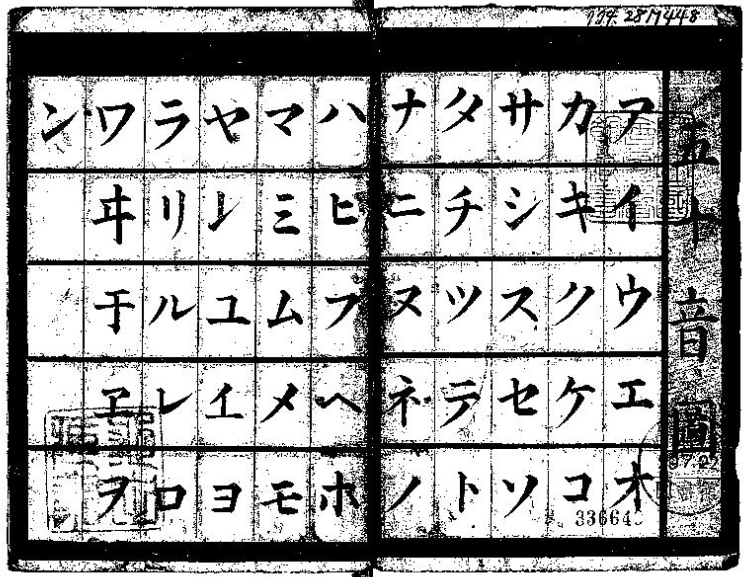
\includegraphics[scale=0.20]{Gojuon000.png}\\
  Katakana Letter Archaic YE =「\texttt{𛄡}」\\
  {\footnotesize defined in Unicode 14.0 (2021)}\\
\vskip1.5ex
\tiny
Ref. http://www.unicode.org/L2/L2019/19381-missing-kana.pdf\\
https://dl.ndl.go.jp/info:ndljp/pid/993592
\end{center}

\end{column}
\end{columns}

\end{frame}

% - - % - - % - - % - - % - - % - - % - - % - - % - - %

\begin{frame}[fragile]{Japanese, Archaic Kana}

\begin{columns}
\begin{column}{55mm}

\setmonofont{mkanaplus-regular.ttf}[Language=Japanese,Script=CJK]
\setsansfont{mkanaplus-regular.ttf}[Language=Japanese,Script=CJK]
\begin{exampleblock}{Archaic Kana Inputs in *.tex}
\begin{Verbatim}[%
  fontfamily=tt,
  fontsize=\fontsize{8.0}{8.0},
  commandchars=!<>]
𛀁\index{𛀁}. % !colRd!-Hiragana Archaic YE
                       %  or !colRd!-Hentaigana E-1
𛄟\index{𛄟}. % Hiragana WU
𛄠\index{𛄠}. % Katakana YI
𛄡\index{𛄡}. % Katakana YE
𛄢\index{𛄢}. % Katakana WU
!colGy!-...
\end{Verbatim}
\end{exampleblock}
\begin{exampleblock}{Dictionary: \footnotesize ``𛀁'' is Hentaigana E-1}
\begin{Verbatim}[%
  fontfamily=tt,
  fontsize=\fontsize{8.0}{8.0},
  commandchars=!<>]
!colRd!-𛀁                  え
\end{Verbatim}
\end{exampleblock}
\begin{exampleblock}{Style: \footnotesize ``𛀁'' is Hiragana Archaic YE}
\begin{Verbatim}[%
  fontfamily=tt,
  fontsize=\fontsize{8.0}{8.0},
  commandchars=!<>]
icu_rules "!colRd!-&ゆ<𛀁<<<𛄡<よ!colBk!-"
\end{Verbatim}
\end{exampleblock}
\end{column}

\begin{column}{38mm}
\begin{center}
\fbox{%
  \includegraphics[scale=0.48]{jp02-02-crop.pdf}%
}
\end{center}
\end{column}

\begin{column}{38mm}
\begin{center}
\fbox{%
  \includegraphics[scale=0.48]{jp03-02-crop.pdf}%
}
\end{center}
\end{column}
\end{columns}

\end{frame}

% - - % - - % - - % - - % - - % - - % - - % - - % - - %

\setmonofont{Noto Sans Mono CJK KR}[Language=Korean,Script=Hangul]
\begin{frame}[fragile]{Korean, Modarn / Archaic Hangul}
\begin{korean}

\begin{columns}
\begin{column}{18mm}
\begin{block}{\hfil ideograph\hfil\\\hfil\scriptsize 한자\hfil}
\begin{center}
  \LARGE \colBl 日
\end{center}
\end{block}
\end{column}
\begin{column}{18mm}
\begin{block}{\hfil modarn\hfil\\\hfil\scriptsize 현대 한글\hfil}
\begin{center}
\begin{tabular}{c}
  \LARGE {\colBl 일} \\[0.5mm]
  \scriptsize U+C77C
\end{tabular}
\end{center}
\end{block}
\end{column}
\begin{column}{87mm}
\begin{block}{\hfil archaic, composed / decomposed\hfil\\\hfil\scriptsize 옛 한글, 완성형 / 조합형 (完成型 / 組合型)\hfil}
\begin{tabular}{cccccccc}
\multirow{2}{*}{\LARGE{\colBl ᅀᅵᇙ〮} =~} & \Large{\colBl ᅀ} & \multirow{2}{*}{+} & \Large{\colBl ᅵ} & \multirow{2}{*}{+}& \Large{\colBl ᇙ} & \multirow{2}{*}{+} & \Large{\colBl 〮} \\[2mm]
                                & \scriptsize{\parbox[u]{7.8mm}{\hfil U+1140\hfil\\\hspace*{0.8mm}첫소리\\\hspace*{1.7mm}初聲}} &&
                                  \scriptsize{\parbox[u]{11.3mm}{\hfil U+1175\hfil\\가운뎃소리\\\hspace*{2.7mm}中聲}} &&
                                  \scriptsize{\parbox[u]{7.8mm}{\hfil U+11D9\hfil\\\hspace*{0.8mm}끝소리\\\hspace*{1.7mm}終聲}} &&
                                  \scriptsize{\parbox[u]{7.8mm}{\hfil U+302E\hfil\\\hspace*{1.7mm}방점\\\hspace*{1.7mm}傍點}}
\end{tabular}
\end{block}
\end{column}
\end{columns}
\vskip3ex
\begin{center}
\begin{tabular}{c|cc|ccc}
        & Unicode block     &     style       & upmendex    &  upLaTeX & XeLaTeX                \\\hline\hline
modarn                      & Hangul Syllables & composed    & ✓             &   ✓     &  ✓ \\
\footnotesize{ex. 일}       & Hangul Jamo      & decompopsed & ✓             &  N.A.    &  ✓ \\\hline
archaic                     & Private Use Area & composed    & \footnotesize{via dictionary} &  ✓ & ✓ \\
\footnotesize{ex. ᅀᅵᇙ〮} & Hangul Jamo      & decomposed  & ✓             &  N.A.    &  ✓ \\\hline
\end{tabular}
\end{center}

% 일  U+C77C  \scriptsize{(完成型)}\scriptsize{(組合型)}
%
% 한
% 한
% 
% ᅀᆞᇙ

\end{korean}
\end{frame}

% - - % - - % - - % - - % - - % - - % - - % - - % - - %

\setmonofont{Noto Sans Mono CJK KR}[Language=Korean,Script=Hangul]
\begin{frame}[fragile]{Korean Hangul}

\begin{columns}
\begin{column}{70mm}

\setmonofont{Noto Sans Mono CJK KR}
\begin{exampleblock}{Hangul Inputs in *.tex}
\begin{Verbatim}[%
  fontfamily=tt,
  fontsize=\fontsize{8.0}{8.0},
  commandchars=!<>]
쓰\index{쓰 (composed)}.
쓰\index{쓰 (decomposed)}.

ᄊ!,ᆞ\index{ᄊ!,ᆞ (archaic)}.
ᄊ!,ᆞ!,〯\index{ᄊ!,ᆞ!,〯 (archaic with tone mark)}.
ᄊᆞ\index{ᄊᆞ (Hanyang PUA)}.
!colGy!-...
\end{Verbatim}
\end{exampleblock}
\begin{exampleblock}{Dictionary for PUA code *.dic}
\begin{Verbatim}[%
  fontfamily=tt,
  fontsize=\fontsize{8.0}{8.0},
  commandchars=!<>]
!colRd!-Hanyang!;PUA!;code!colBk!-  !colRd!-decomposed!colBk!-
ᄊᆞ                ᄊ!,ᆞ
ᄊᆡ                ᄊ!,ᆡ
!colGy!-...
\end{Verbatim}
\end{exampleblock}
\end{column}

\begin{column}{60mm}
\begin{center}
\fbox{%
  \includegraphics[scale=0.48]{ko03-02-crop.pdf}%
}%
\end{center}
\end{column}
\end{columns}

\end{frame}


% - - % - - % - - % - - % - - % - - % - - % - - % - - %

\subsection{Devanagari, Thai, Arabic, Hebrew}

\setmonofont{Noto Sans Mono}
\begin{frame}[fragile]{Devanagari \& Thai}

\begin{columns}
\begin{column}{50mm}

%\setsansfont{Noto Sans}
\setmonofont{Noto Serif Devanagari}[Language=Hindi,Script=Devanagari]
\setmainfont{Noto Sans Mono}
\setsansfont{Noto Sans}
\begin{exampleblock}{Hindi Inputs in *.tex}
\begin{Verbatim}[%
  fontfamily=tt,
  fontsize=\fontsize{8.0}{8.0},
  commandchars=!<>,
  baselinestretch=1.5]
फूल!,!sffamily!-\index{!ttfamily!-!,फूल!,!sffamily!-}
चिड़िया!,!sffamily!-\index{!ttfamily!-!,चिड़िया!,!sffamily!-}
हवा!,!sffamily!-\index{!ttfamily!-!,हवा!,!sffamily!-}
चांद!,!sffamily!-\index{!ttfamily!-!,चांद!,!sffamily!-}
!colGy!-...
\end{Verbatim}
\end{exampleblock}
\setmonofont{Noto Serif Thai}[Language=Thai,Script=Thai]
\setmainfont{Noto Sans Mono}
\setsansfont{Noto Sans}
%\setsansfont{Noto Sans CJK JP}[Language=Japanese,Script=CJK]
\begin{exampleblock}{Thai Inputs in *.tex}
\begin{Verbatim}[%
  fontfamily=tt,
  fontsize=\fontsize{8.0}{8.0},
  commandchars=!<>,
  baselinestretch=1.5]
ดอกไม้!,!sffamily!-\index{!ttfamily!-!,ดอกไม้!,!sffamily!-}
นก!,!sffamily!-\index{!ttfamily!-!,นก!,!sffamily!-}
ลม!,!sffamily!-\index{!ttfamily!-!,ลม!,!sffamily!-}
ดวงจันทร์!,!sffamily!-\index{!ttfamily!-!,ดวงจันทร์!,!sffamily!-}
!sffamily!colGy!-...
\end{Verbatim}
\end{exampleblock}
\end{column}

\begin{column}{79mm}

\begin{columns}
\begin{column}{39mm}
\begin{center}
\fbox{%
  \includegraphics[scale=0.48]{hi00-02-crop.pdf}%
}\\[2mm]%
Hindi
\end{center}
\end{column}

\begin{column}{39mm}
\begin{center}
\fbox{%
  \includegraphics[scale=0.48]{th00-02-crop.pdf}%
}\\[2mm]%
Thai
\end{center}
\end{column}
\end{columns}
\vspace{2mm}
\begin{center}
{\footnotesize Typeset by XeLaTeX}
\end{center}
\end{column}

\end{columns}

\end{frame}


% - - % - - % - - % - - % - - % - - % - - % - - % - - %

\setmonofont{Noto Sans Mono}
\begin{frame}[fragile]{Arabic \& Hebrew}

\begin{columns}
\begin{column}{50mm}

%\setsansfont{Noto Sans}
%\setmonofont{Noto Serif Devanagari}[Language=Hindi,Script=Devanagari]
\setmonofont{DejaVu Sans}[Script=Arabic]
\setmainfont{Noto Sans Mono}
\setsansfont{Noto Sans}
\begin{exampleblock}{Arabic Inputs in *.tex}
\begin{Verbatim}[%
  fontfamily=tt,
  fontsize=\fontsize{8.0}{8.0},
  commandchars=!<>,
  baselinestretch=1.5]
زهرة!,!sffamily!-\index{!ttfamily!-!,زهرة!,!sffamily!-}
عصفور!,!sffamily!-\index{!ttfamily!-!,عصفور!,!sffamily!-}
ريح!,!sffamily!-\index{!ttfamily!-!,ريح!,!sffamily!-}
القمر!,!sffamily!-\index{!ttfamily!-!,القمر!,!sffamily!-}
!colGy!-...
\end{Verbatim}
\end{exampleblock}

%\setmonofont{Noto Serif Hebrew}[Script=Hebrew]
\setmonofont{DejaVu Sans}[Script=Hebrew]
\setmainfont{Noto Sans Mono}
\setsansfont{Noto Sans}
\begin{exampleblock}{Hebrew Inputs in *.tex}
\begin{Verbatim}[%
  fontfamily=tt,
  fontsize=\fontsize{8.0}{8.0},
  commandchars=!<>,
  baselinestretch=1.5]
פֶּרַח!,!sffamily!-\index{!ttfamily!-!,פֶּרַח!,!sffamily!-}
ציפור!,!sffamily!-\index{!ttfamily!-!,ציפור!,!sffamily!-}
רוּחַ!,!sffamily!-\index{!ttfamily!-!,רוּחַ!,!sffamily!-}
ירח!,!sffamily!-\index{!ttfamily!-!,ירח!,!sffamily!-}
!colGy!-...
\end{Verbatim}
\end{exampleblock}

\end{column}

\begin{column}{79mm}

\begin{columns}
\begin{column}{39mm}
\begin{center}
\fbox{%
  \includegraphics[scale=0.48]{ar00-02-crop.pdf}%
}\\[2mm]%
Arabic
\end{center}
\end{column}

\begin{column}{39mm}
\begin{center}
\fbox{%
  \includegraphics[scale=0.48]{he00-02-crop.pdf}%
}\\[2mm]%
Hebrew
\end{center}
\end{column}
\end{columns}
\vspace{2mm}
\begin{center}
{\footnotesize R-to-L typeset by XeLaTeX.\\
\textbf{upmendex} processes only indexing.}
\end{center}
\end{column}
\end{columns}

\end{frame}

% - - % - - % - - % - - % - - % - - % - - % - - % - - %

\selectlanguage{japanese}
\selectbackgroundlanguage{japanese}
\setmainfont{Noto Serif CJK JP}[Language=Japanese,Script=CJK]
\setsansfont{Noto Sans CJK JP}[Language=Japanese,Script=CJK]
\setmonofont{Noto Sans Mono CJK JP}

%\subsection{Symbol, Number}
\begin{frame}{Symbol, Number}

\begin{center}
\scriptsize
\begin{tabular}{c|cc|c}
Script     & charType & example & treatment by upmendex \\\hline\hline
Latin      & \texttt{\colBl Lu, Ll, Lo,} ... : letters & ABCabcAaⓐ & directly pass to ICU collator \\
Greek      & \texttt{\colBl Lu, Ll, Lo,} ... : letters & ΑΒΓαβγ & direct \\
Cyrillic   & \texttt{\colBl Lu, Ll, Lo,} ... : letters & АБВабв  & direct \\
%Thai       & Lo, \ldots         : letters & \begin{thai}กขฃคฅฆ\end{thai} & direct \\
Kana       & \texttt{\colBl Lo} : other letter & あいうアア㋐㌀ & direct \\
Hangul     & \texttt{\colBl Lo} : other letter & \begin{korean}가나다ᄁ㉡㉰㉼\end{korean} & direct \\
Hanzi      & \texttt{\colBl Lo} : other letter & 花鳥風月 & lookup dictionary or direct \\
---        & \texttt{\colBl Lm} : modifier letter   & ー゙゚ー & direct \\\hline
\multirow{2}{*}{Number}  & \texttt{\colBl Nd} : dicimal digit number & 012012 & direct \\
           & \texttt{\colBl No}      : other number & ¹²③❹➄➏🄈⑻⒐ & lookup dictionary or direct \\\hline
\multirow{5}{*}{Symbol}  & \texttt{\colBl Sk} : modifier symbol   & ¨¯´^`゛゜& direct \\
           & \texttt{\colBl Sm} : math symbol       & ÷▷♯ & lookup dictionary or direct \\
           & \texttt{\colBl So}               : other symbol      & ☃〠☎♥⚽⚾ & lookup dictionary or direct \\
           & \texttt{\colBl Sc}               : currency symbol   & €\$$¢£¥¥₩₩ & lookup dictionary or direct \\
           & \texttt{\colBl Po, Pd, Mn, Me,} ... : other punctuation etc. & ⁈⁉¡¿†\#§¶— & direct \\\hline
---        & \texttt{\colBl Cc}                 : control character & ESC, BS, DEL & ignore \\
---        & \texttt{\colBl Cf}                 : format character  & BOM, RLM & diect \\
others     & \texttt{\colBl Lo,} etc. (unknown scripts)             &  & lookup dic or direct (option ``-f'') or ignore \\\hline
\end{tabular}
\end{center}
\begin{center}
Characters are classified by Unicode ``charType''
\end{center}

\end{frame}
%€\$$¢££¥¥₩₩

% - - % - - % - - % - - % - - % - - % - - % - - % - - %

\section{Multilingual environment}

\setmonofont{Noto Sans Mono CJK JP}
\begin{frame}[fragile]{Multilingual Environment with upLaTeX/pxbabel}
\begin{columns}
\begin{column}{84mm}
\begin{exampleblock}{Block Setting for Scripts in Style File *.ist}
\makeatletter
%\def\verbatim@font{\footnotesize\textjapanese}
\def\verbatim@font{\fontsize{7.5}{7.5}\selectfont\textjapanese}
\makeatother
\begin{Verbatim}[%
  fontfamily=tt,
  fontsize=\fontsize{7.5}{7.5},
  commandchars=!<>]

script_preamble   cyrillic "\n!colRd!-\\fontencoding{T2A}\\selectfont!colBk!-"
script_postamble  cyrillic "\n!colRd!-\\fontencoding{T1}\\selectfont!colBk!-"
script_preamble   hangul   "\n!colRd!-\\begin{otherlanguage}{korean}!colBk!-"
script_postamble  hangul   "\n!colRd!-\\end{otherlanguage}!colBk!-"
script_preamble   hanzi    "\n!colRd!-\\begin{otherlanguage}{tchinese}!colBk!-"
script_postamble  hanzi    "\n!colRd!-\\end{otherlanguage}!colBk!-"

\end{Verbatim}
\end{exampleblock}
\end{column}
\begin{column}{60mm}
\begin{exampleblock}{Output *.ind}
\begin{Verbatim}[%
  fontfamily=tt,
  fontsize=\fontsize{7.5}{7.5},
  commandchars=!<>]
\centerline{\bfseries --- С ---}\par\nobreak
  \item София\leaders\hbox{~}\hfill 1
!colGy!-...
!colRd!-\fontencoding{T1}\selectfont

  \indexspace

\centerline{--- サ ---}\par\nobreak
  \item さいたま\leaders\hbox{~}\hfill {1}
  \item 札幌\leaders\hbox{~}\hfill {1}
!colGy!-...
!colRd!-\begin{otherlanguage}{korean}

  \indexspace

\centerline{\bfseries --- ㅂ ---}\par\nobreak
  \item 부산(釜山)\leaders\hbox{~}\hfill 1
!colGy!-...
!colRd!-\end{otherlanguage}
\end{Verbatim}
\end{exampleblock}
\end{column}
\end{columns}

\end{frame}

% - - % - - % - - % - - % - - % - - % - - % - - % - - %

%\setmainfont{DejaVu Sans}
%\setsansfont{DejaVu Sans}
%\setmainfont{Noto Serif Hebrew}[Script=Hebrew]
%\setsansfont{Noto Serif Hebrew}[Script=Hebrew]
%\setmonofont{Noto Serif Hebrew}[Script=Hebrew]
%\setmainfont{SILEOT.ttf}
%\setsansfont{SILEOT.ttf}
%\setmonofont{SILEOT.ttf}
\begin{frame}[fragile]{Multilingual Environment with polyglossia}
\begin{columns}
\begin{column}{72mm}
\begin{exampleblock}{Block Setting for Scripts in Style File *.ist}
\setmonofont{Noto Sans Mono CJK JP}
\begin{Verbatim}[%
  fontfamily=tt,
  fontsize=\fontsize{7.5}{7.5},
  commandchars=!<>]

script_preamble   cyrillic "\n!colRd!-\\begin{russian}!colBk!-"
script_postamble  cyrillic "\n!colRd!-\\end{russian}!colBk!-"
script_preamble   kana     "\n!colRd!-\\begin{japanese}!colBk!-"
script_postamble  kana     "\n!colRd!-\\end{japanese}!colBk!-"
script_preamble   hangul   "\n\n!colRd!-\\begin{korean}!colBk!-"
script_postamble  hangul   "\n!colRd!-\\end{korean}!colBk!-"
script_preamble   hebrew   "\n!colRd!-\\begin{hebrew}!colBk!-"
script_postamble  hebrew   "\n!colRd!-\\end{hebrew}!colBk!-"

\end{Verbatim}
\end{exampleblock}
\end{column}

\begin{column}{72mm}
\begin{exampleblock}{Output *.ind}
\setmonofont{Noto Sans Mono CJK JP}
\begin{Verbatim}[%
  fontfamily=tt,
  fontsize=\fontsize{7.5}{7.5},
  commandchars=!<>]
!colGy!-...
!colRd!-\end{japanese}

!colRd!-\begin{korean}

  \indexspace

\centerline{--- ㄷ ---}\par\nobreak
  \item 대구(大邱)\leaders\hbox{~}\hfill {1}
!colGy!-...
!colRd!-\end{korean}
\end{Verbatim}
%\setmainfont{DejaVu Sans}
\setsansfont{SILEOT.ttf}
%\setmonofont{SILEOT.ttf}
%\setmonofont{Noto Serif Hebrew}[Script=Hebrew]
\setmonofont{DejaVu Sans}[Script=Hebrew]
%\setmainfont{Noto Sans Mono}
%\setsansfont{Noto Sans}
\begin{hebrew}
\begin{Verbatim}[%
  fontfamily=tt,
  fontsize=\fontsize{7.5}{7.5},
  commandchars=!<>]
!colRd!-\begin{hebrew}

  \indexspace

\centerline{--- א ---}\par\nobreak
  \item אשדוד!,\leaders\hbox{~}\hfill {2}
!colGy!-...
!colRd!-\end{hebrew}
\end{Verbatim}
\end{hebrew}
\end{exampleblock}
\end{column}
\end{columns}

\end{frame}

% - - % - - % - - % - - % - - % - - % - - % - - % - - %

\begin{frame}[fragile]{Output of Multilingual Index}
\begin{columns}

\begin{column}{60mm}
\begin{center}
\fbox{%
  \includegraphics[scale=0.41]{city1-03-crop.pdf}%
}\\[1mm]%
\footnotesize with upLaTeX \& pxbabel
\end{center}
\end{column}

\begin{column}{60mm}
\begin{center}
\fbox{%
  \includegraphics[scale=0.41]{city0-03-crop.pdf}%
}\\[1mm]%
\footnotesize with XeLaTeX \& polyglossia
\end{center}
\end{column}
\end{columns}

\end{frame}

% - - % - - % - - % - - % - - % - - % - - % - - % - - %

\section{Benchmark}
\begin{frame}{Benchmark}

\begin{center}
\footnotesize
\begin{tabular}{c|c|c|c|c}
            & makeindex & mendex      & upmendex            & xindy   \\\hline\hline
internal encoding & 8bit 1byte & EUC-JP    & UTF-16         & Unicode \\
Collator    & locale    & ASCII, Kana & ICU collator        &         \\\hline
Latin       & ✓        & ✓ ASCII    & Lang:37, Locale:62  & Lang:32 \\
Greek       &           &             & Lang:1, Locale:1    & Lang:1 \\
Cyrillic    &           &             & Lang:9, Locale:9    & Lang:6 \\\hdashline
Chinese     &           &             & Lang:1, Locale:4    &  \\
\multirow{2}{*}{Japanese} & & \multirow{2}{*}{✓ (Yomi, Dict)} & ✓ (Yomi, Dict) & \\
            &           &             & Lang:1, Locale:2    & \\
Korean      &           &             & Lang:1, Locale:3    & \\\hdashline
Devanagari  &           &             & Lang:3, Locale:3    & \\
Thai        &           &             & Lang:1, Locale:1    & \\
Arabic      &           &             & Lang:6, Locale:7    & \\
Hebrew      &           &             & Lang:2, Locale:3    & Lang:1  \\\hdashline
Other       &           &             &                     & Lang:4  \\\hline
Total       &           & Lang:2      & Lang:60, Locale:95  & Lang:44 \\\hline
\end{tabular}
\end{center}

\end{frame}

% - - % - - % - - % - - % - - % - - % - - % - - % - - %

\begin{frame}{Languages by Number of Native Speakers}

\setlength\dashlinedash{0.5pt}
\setlength\dashlinegap{1.0pt}

\begin{center}
\scriptsize
\begin{tabular}{ccc|r|cccc}
  & Language    & Script & speakers & ICU & polyglossia & upmendex & xindy \\\hline\hline
1 & Chinese     & {\colRd Hanzi     } & 1,370,000,000 & ✓ &    & ✓ &    \\
2 & Engish      & Latin      &   530,000,000 & ✓ & ✓ & ✓ & ✓ \\
3 & Hindi       & {\colBl Devanagari} &   490,000,000 & ✓ & ✓ & ✓ &    \\
4 & Spanish     & Latin      &   420,000,000 & ✓ & ✓ & ✓ & ✓ \\
5 & Arabic      & {\colGn Arabic    } &   230,000,000 & ✓ & ✓ & ✓ &    \\\hdashline
6 & Bengali     & {\colBl Bengali   } &   220,000,000 & ✓ & ✓ &    &    \\
7 & Portuguese  & Latin      &   215,000,000 & ✓ & ✓ & ✓ & ✓ \\
8 & Russian     & Cyrillic   &   180,000,000 & ✓ & ✓ & ✓ & ✓ \\
9 & Japanese    & {\colRd Kana \& Hanzi } &   134,000,000 & ✓ & ✓ & ✓ &    \\
10 & German     & Latin      &   130,000,000 & ✓ & ✓ & ✓ & ✓ \\\hline
11 & French     & Latin      &   123,000,000 & ✓ & ✓ & ✓ & ✓ \\
12 & Punjabi    & {\colBl Gurmukhi  } &    90,000,000 & ✓ &    &    &    \\
13 & Javanese   & Latin      &    75,000,000 & ✓ & ✓ & ✓ &    \\
14 & Korean     & {\colRd Hangul    } &    75,000,000 & ✓ & ✓ & ✓ &    \\
15 & Vietnamese & Latin      &    70,000,000 & ✓ & ✓ & ✓ & ✓ \\\hdashline
16 & Telugu     & {\colBl Telugu    } &    70,000,000 & ✓ & ✓ &    &    \\
17 & Marathi    & {\colBl Devanagari} &    68,000,000 & ✓ & ✓ & ✓ &    \\
18 & Tamil      & {\colBl Tamil     } &    74,000,000 & ✓ & ✓ &    &    \\
19 & Persian    & {\colGn Arabic    } &    46,000,000 & ✓ & ✓ & ✓ &    \\
20 & Urdu       & {\colGn Arabic    } &    61,000,000 & ✓ & ✓ & ✓ &    \\\hline
\end{tabular}
\\
{\tiny Ref. https://ja.wikipedia.org/wiki/ネイティブスピーカーの数が多い言語の一覧}
\end{center}
\end{frame}

% - - % - - % - - % - - % - - % - - % - - % - - % - - %

\begin{frame}{Languages used on the Internet}

\setlength\dashlinedash{0.5pt}
\setlength\dashlinegap{1.0pt}

\begin{columns}
\begin{column}{69mm}
\begin{center}
\scriptsize
%\tiny
\begin{tabular}{cc@{~}c@{~}c|c@{~~}c@{~~}c@{~~}c}
  & Language & share & Script & ICU & pg & upm & xnd\\\hline\hline
1 & English & 63.4~\%     &   Latin &  root    & ✓ & ✓ & ✓  \\
2 & Russian & 7.1~\%      &   Cyrillic & ru    & ✓ & ✓ & ✓  \\
3 & Spanish & 3.9~\%      &   Latin &    es    & ✓ & ✓ & ✓  \\
4 & German & 3.7~\%       &   Latin &    de    & ✓ & ✓ & ✓  \\
5 & Turkish & 3.5~\%      &   Latin &    tr    & ✓ & ✓ & ✓  \\\hdashline
6 & Persian & 2.5~\%      &   {\colGn Arabic } &   fa    & ✓ & ✓ &     \\
7 & French & 2.0~\%       &   Latin &    root  & ✓ & ✓ & ✓  \\
8 & Japanese & 1.9~\%     &   {\colRd Kana   } &   ja    & ✓ & ✓ &     \\
9 & Portuguese & 1.8~\%   &   Latin &    pt    & ✓ & ✓ & ✓  \\
10 & Chinese & 1.3~\%     &   {\colRd Hanzi  } &   zh    &    & ✓ &     \\\hline
11 & Vietnamese & 1.3~\%  &   Latin &    vi    & ✓ & ✓ & ✓  \\
12 & Italian & 1.0~\%     &   Latin &    root  & ✓ & ✓ & ✓  \\
13 & Arabic & 0.9~\%      &   {\colGn Arabic } &   ar    & ✓ & ✓ &     \\
14 & Polish & 0.9~\%      &   Latin &    pl    & ✓ & ✓ & ✓  \\
15 & Greek & 0.7~\%       &   Greek &    el    & ✓ & ✓ & ✓  \\\hdashline
16 & Dutch & 0.7~\%       &   Latin &    nl    & ✓ & ✓ & ✓  \\
17 & Indonesian & 0.7~\%  &   Latin &    root  & ✓ & ✓ &     \\% polyglossia では malayのvariant
18 & Korean & 0.6~\%      &   {\colRd Hangul } &   ko    & ✓ & ✓ &     \\
19 & Czech & 0.4~\%       &   Latin &    cs    & ✓ & ✓ & ✓  \\
20 & Thai & 0.4~\%        &   {\colBl Thai   } &   th    & ✓ & ✓ &     \\\hline
\end{tabular}
\end{center}
\end{column}
\begin{column}{83mm}
\begin{center}
\scriptsize
%\tiny
\begin{tabular}{cc@{~}c@{~}c|c@{~~}c@{~~}c@{~~}c}
  & Language & share & Script & ICU & pg & upm & xnd\\\hline\hline
21 & Ukrainian & 0.3~\%   &   Cyrillic & uk    & ✓ & ✓ & ✓  \\
22 & Hebrew & 0.3~\%      &   {\colGn Hebrew } &   he    & ✓ & ✓ & ✓  \\
23 & Swedish & 0.3~\%     &   Latin &    sv    & ✓ & ✓ & ✓  \\
24 & Romanian & 0.3~\%    &   Latin &    ro    & ✓ & ✓ & ✓  \\
25 & Hungarian & 0.3~\%   &   Latin &    hu    & ✓ & ✓ & ✓  \\\hdashline
26 & Danish & 0.2~\%      &   Latin &    da    & ✓ & ✓ & ✓  \\
27 & Slovak & 0.2~\%      &   Latin &    sk    & ✓ & ✓ & ✓  \\
28 & Serbian & 0.2~\%     &   Latn, Cyrl & sr  & ✓ & ✓ & ✓  \\ %Latin, Cyrillic
29 & Bulgarian & 0.1~\%   &   Cyrillic & bg    & ✓ & ✓ & ✓  \\
30 & Finnish & 0.1~\%     &   Latin &    fi    & ✓ & ✓ & ✓  \\\hline
31 & Croatian & 0.1~\%    &   Latin &    hr    & ✓ & ✓ & ✓  \\
32 & Lithuanian & 0.1~\%  &   Latin &    lt    & ✓ & ✓ & ✓  \\
33 & Norwegian (Bokmål)   & 0.1~\% &   Latin &    nb & ✓ & ✓ & ✓ \\
34 & Hindi & 0.1~\%       &   {\colBl Devanagari} & hi  & ✓ & ✓ &    \\
35 & Norwegian (nynorsk)  & 0.1~\% &   Latin &    nn & ✓ & ✓ & ✓ \\\hdashline
36 & Slovenian & 0.1~\%   &   Latin &    sl    & ✓ & ✓ & ✓  \\ % Slovenian
37 & Latvian & 0.1~\%     &   Latin &    lv    & ✓ & ✓ & ✓  \\ %(1.02)
38 & Estonian & 0.1~\%    &   Latin &    et    & ✓ & ✓ & ✓  \\%(1.02)
39 & Azerbaijani & < 0.1~\% & Latin &    az    &    & ✓ &    \\ %Latin, ペルシャ文字, Cyrillic
40 & Catalan & < 0.1~\%   &   Latin &    root  & ✓ & ✓ &     \\\hline
\end{tabular}
\end{center}
\end{column}
\end{columns}
%\\
{\tiny Ref. https://ja.wikipedia.org/wiki/インターネットにおける言語の使用}
\end{frame}

% - - % - - % - - % - - % - - % - - % - - % - - % - - %

\begin{frame}{ToDo}

\begin{center}
  \begin{itemize}
  \item Support more scripts\\
     \begin{itemize}
      \item Bengali, Telugu, Tamil, Malayalam, Kannada, Gujarati, Sinhala, etc.
      \item Khmer, Lao, Myanmar (Burmese)
      \item Tibetan, Mongolian
      \item Armenian, Georgian
      \item Ethiopic (Amharic)
      \item etc.
     \end{itemize}
  \item Support more locales\\
     \begin{itemize}
      \item Latin: Sorbian, Hausa, Kalaallisut, Breton, Uzbek
      \item etc.
     \end{itemize}
  \item Add style options\\
     \begin{itemize}
      \item \texttt{script\_head}
     \end{itemize}
  \end{itemize}
\vskip1.5ex
{\Large Feedback is welcome}
\end{center}

\end{frame}

% - - % - - % - - % - - % - - % - - % - - % - - % - - %

\section{Summary}
\begin{frame}{Summary}

\begin{columns}
\begin{column}{70mm}

I introduced multilingual index processor \textbf{upmendex}.

  \begin{itemize}
  \item Feature\\
  \item Localization: 60 Languages, 12 Scripts
     \begin{itemize}
      \item Latin, Cyrillic, Greek
      \item CJK (Chinese, Japanese, Korean)
      \item Devanagari, Thai, Arabic, Hebrew
      \item Symbol, Number
     \end{itemize}
  \item Multilingualization
     \begin{itemize}
      \item Environment for\\
        upLaTeX/babel \& XeLaTeX/polyglossia
     \end{itemize}
  \end{itemize}
\end{column}

\begin{column}{65mm}

\begin{center}
\fbox{%
  \includegraphics[scale=0.47]{city_texconf-03-cropa.pdf}%
}
\end{center}
\end{column}
\end{columns}

\end{frame}


\end{document}


